textbf{Definition of Markov chains}\\

A discrete Markov Chain is
\begin{itemize}
	\item A discrete-time stochastic process $\{X_n, n=0,1,2... \}$
	\item That takes on a finite or countable number of possible value (discrete state space $S_x$) called "states" and usually denoted by integers without loss of generality
	\item Satisfying the Markov property. That is, for any $i, j, i_0, i_1...i_{n-1} \in S_x = \{ 0,1,....\}$
	$$ \mathbb{P} $$
\end{itemize}


\textbf{Champan-Kolmogorov Equations}\\
For all $n, m \geq 0, i, j \geq 0$ we have

$$P_{ij}^{[n+m]} = \sum_{k\in S_X} P_{ik}^{[n]} P_{kj}^{[m]}$$

Note: $P^{[0]} = I$

\textbf{Transformed transition matrix}\\
Assume that we've entered some states $\mathcal{A}$ by time $m$\\

Then we reset the matrix to:

$$Q_{ij} = \mathbb{P}*(X_{n+1} = j|X_n = i) = \begin{cases} 1 & \text{if }i \in \mathcal{A}, j= i \\ 0 & \text{if }i\in \mathcal{A}, j \neq i \\ P_{ij} & \text{if } i \not \in \mathcal{A} \end{cases}$$

\textbf{Accessible states}\\

State $j$ is said to be accessible from state $i$ denoted by $i \rightarrow j$ if

$$[P^n]_{ij} = P_{ij}^[n] > 0$$
for some $n \geq 0$.\\

\textbf{Communicating states}\\
Two states $i$ and $j$ communicate, denoted by $i \leftrightarrow j$ if $i$ is accessible form $j$ and $j$ is accessible from $i$.\\

\textbf{Communication classes}\\
A class $\mathcal{C}$ is a non-empty set of states such that for each state $i \in \mathcal{C}$ $i$ communicates with all $j \in \mathcal{C}$ and does not communicate with any $j \not \in \mathcal{C}$\\

\textbf{Irreducible chain}\\
A markov chain is said to be irreducible if there is only one class, that is if all states communicate with each other.\\

\textbf{Classification of states}\\
State $i$ is said to be
\begin{enumerate}
	\item \textbf{recurrent} if $p_i = 1$
	\item \textbf{transient} if $p_i < 1$
\end{enumerate}

State $i$ is recurrent if $\sum_{n=0}^\infty P_{ii}^[n] = + \infty$\\
and transient if the same sum $< \infty$\\

\textbf{Period}\\
The period of a state $i$ is denoted by $d(i)$ is the greatest common divisor of the values of $n$ for which $P_{ii}^{[n]} > 0$. If the period of the state is 1, the state is aperiodic.\\

In a Markov Chain, all state in a given class has the same period. (Proof slide 235)\\

\textbf{Positive and null recurrent}\\
A state $i$ of a Markov Chain is \textbf{positive recurrent} if its recurrent and $\mathbb{E}(T_{ii}) < +\infty$. It is \textbf{null recurrent} if it is recurrent and $\mathbb{E}(T_{ii}) = + \infty$.\\

\textbf{Ergodic}
A state is said to be \textbf{ergodic} if it is positive-recurrent and aperiodic. A class of ergodic states is known as an ergodic chain. \\

\textbf{Theorem - Ergodic markov Chain}\\

For an ergodic markov chain\\

$$lim_{n \rightarrow \infty} P_{ij}^{[n]} \text{ exists for all } j$$

and is independent of $i$. Furthermore, letting

$$\pi_j = \lim_{n \rightarrow \infty} P_{ij}^{[n]}$$

then $\pi = (\pi_0, \pi_1, \pi_2,...)$ is the unique nonnegative solution of the system of equations

$$\begin{cases} \pi_j = \sum_{[i\in S_x]} \pi_i P_{ij} \\ 1 = \sum_{[i \in S_X]} \pi_j  \end{cases}$$

\textbf{Stationary distribution}\\

Take the law of total probability:\\

$$\mathbb{P}(X_{n+1}) = \sum_{i \in S_X} \mathbb{P}(X_{n+1} = j|X_n = i) \mathbb{P}(X_n = i)$$

Suppose that the distribution of $X_n$ is $\pi$. Then

$$\mathbb{P}(X_{n+1} = j) = \sum_{i \in S_X} P_{ij} \pi_j = \pi_j $$

The vector $\pi$ is called the stationary distribution. It is also the long run probability of time that the process will be in the state $j$.

\textbf{Limiting probabilities}\\

For examples, see slides 249-253

\textbf{Non Ergodic cases}

If the chain is ergodic then $P^n$ converges as $n \rightarrow +\infty$ and there is one single stationary distribution $\pi$, which is the unique solution of $\pi = \pi P$\\

Non ergodic means
\begin{itemize}
	\item not reducible
	\item periodic
	\item null recurrent
\end{itemize}

A non-irreducible chain means with one recurrent class and some transient classes meansthat it experiences a:

\begin{itemize}
	\item Stationary distribution = long term behaviour of chain
	\item transient classes play a role only for a finite number of transitions
	\item After a certain number of transitions the chain enters a recurrent class and never leaves it.
\end{itemize}

\textbf{Ergodic theorem}\\

Let $\{X_n, n \geq 0 \}$ be an ergodic Markov Chain with stationary probabilities $\pi_j \geq 0$. Let $r$ be a bounded function: $S_X \rightarrow R \subset \mathbb{R}$. Then with probability 1

$$ \lim_{N \rightarrow \infty} \frac{1}{N} \sum_{n=0}^{N-1} r(X_n) = \sum_{j \in S_X} r(j) \pi_j $$
for any starting value $X_0$.

Loosely time average = space average\\

In fact most of the limit theorems for sums of independent random variables essentially holds true for sums of dependent random variables, provided that the dependance isn't too strong.\\

\textbf{Canonical form}\\
You can always rearrange states of the chain to have this form

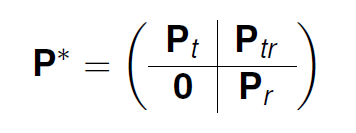
\includegraphics[scale = 0.3]{canonical}\\

If $R$ is the number of recurrent states then\\
\begin{itemize}
	\item $P_t$ is the $(T \times T)$ matrix of transitions from a transient state to a transient state.\\
	\item $P_{tr}$ is the matrix of transitions from a transient state to a recurrent state
	\item $P_r$ is the matrix of transitions from a recurrent state to a recurrent state.
\end{itemize}

$P*$ is called the canonical form of $P$.\\

\textbf{How long will the chain be in transient states before its absorbed?}\\

Conditioning on first transition from $i$ we get:
$$S_{ij} = \delta_{ij} + \sum_{k=1}^{T+R} P_{ik}* S_{kj} = \delta_{ij} + \sum_{k=1}^T [P_t]_{ik} +S_{ij}$$

where $\delta_{ij}$ is the Kronecker delta. $\delta_{ij} = \begin{cases}1 & i = j \\ 0 & i \neq j \end{cases}$\\

In Matrix notation\\

$$S = I + P_tS$$
so:

$$S = (I - P_T)^{-1}$$

It follows that $S$ can be referred to as the \textbf{fundamental matrix}.\\

\textbf{On average how long will it take for the chain to be absorbed?}\\

Let $\sigma_i$ be the amount of time before the chain is absorbed, given the chain is now in transient state $i$.
$$\sigma_i = \sum_{j=1}^T S_{ij}$$

If $\sigma = (\sigma_1 \sigma_2.... \sigma_T)^t$ we have

$$\sigma = Se = (1 - P_t)^{-1} e$$

For absorption examples see slides 283-289

\textbf{Probability generating function}\\

The probability generating function of a non negative integer valued random value $X$ iis defined by

$$G_X(s) = \mathbb{E}(s^X) = \sum_{j=0}^{+\infty} s^j \mathbb{P}(X = j)$$

The pgf $G_X(s)$ is such that
\begin{enumerate}
	\item It exists for all values $s \in [0,1]$ as $\sum_{j} \mathbb{P}(X = j) = 1$
	\item It is continusous, non decreasing and convex over $[0,1]$
	\item $G_X(0) = \mathbb{P}(X=0)$ and $G_X(1) = 1$
	\item It is infinitely many times differentiable over $[0,1]$ 
	\item (See slide 292)
	\item (See slide 293)
\end{enumerate}

\textbf{Branching process}

The evolution of a total population as time proceeds is called a \textbf{branching process}\\

\textbf{Galton Watson definition of the process}\\

By assumption, $\{ Y_{n,k} \}$ are i.i.d random variables with common probability distribution $\mathbb{P}(Y = j) = p_j$ for $j = 0,1,2...$ and 
	
$$X_{n+1} = \sum_{k=1}^{X_n} Y_{n,k}$$